\section{Structure}\label{sc:structure}
% Intro intro
Based on the analysis in the former sections, the structure of the classes in the problem domain has been visualised in a class diagram (see \autoref{fig:FirstPDClassDiagram}).

\begin{figure}[H]
    \centering
    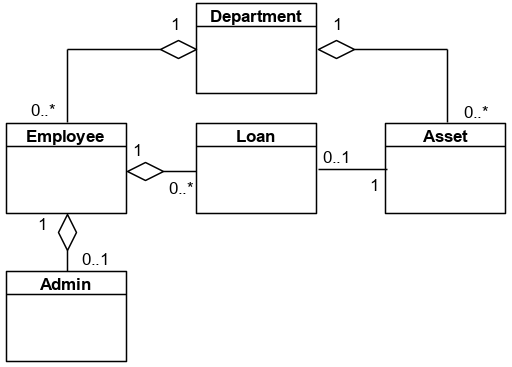
\includegraphics[width=0.6\textwidth]{figures/ClassDiagrams/InitialClassDiagramWithoutTag.png}
    \caption{Class diagram of the classes in the problem domain.}
    \label{fig:FirstPDClassDiagram}
\end{figure}

As described in \autoref{sc:class_activity}, there are six different relevant classes in the problem domain. These classes are: \textit{Employee}, \textit{Admin}, \textit{Department}, \textit{Asset}, and \textit{Loan}. The relations between these have been explained below.
\par

The \textit{Employee} class is an aggregation of the \textit{Admin} class. The structure created by this connection is a role pattern with only one role. The pattern makes it possible for an employee to possess the role of \textit{Admin} dynamically.
\par

The \textit{Department} class aggregates a number of assets and employees, and each of these belong to one department.
\par

The \textit{Employee} class aggregates a number of \textit{Loan} classes, and each loan belongs to one employee. Each instance of the \textit{Loan} class has a association to an asset, and an asset is associated to none or one loan. These connections form a Relation Pattern.

%The \textit{Asset-tag relation} class is created to handle the relation between the \textit{Asset} and \textit{Tag} classes, as multiple assets can be tagged with the same tag and an asset can have multiple tags. The \textit{Asset} class aggregates it, as an asset can contain multiple connections to tags. The aggregation is made to the asset and not the tag, as the tags only function is being connected to assets. The structure is base on the relation pattern. An instance of the \textit{Asset-tag relation} class always connects one asset and one tag, but both the \textit{Tag} and \textit{Asset} classes can be part of multiple asset-tag relations.
\par

With the classes of the problem domain and their interconnecting relations described, the behaviour of the classes can be examined.
\newpage